\title{%
  The terminal
}
\author{Daniel Bosk}
\institute{%
  KTH EECS
}

\mode<article>{\maketitle}
\mode<presentation>{%
  \begin{frame}
    \maketitle
  \end{frame}
}

\mode*


\section{What to learn?}

\subsection{Terminal}

\begin{frame}
  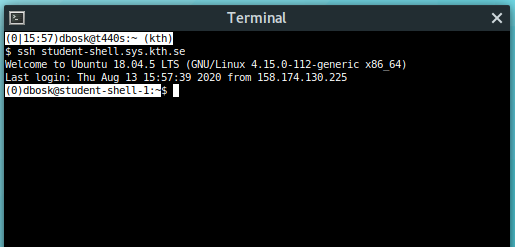
\includegraphics[width=\columnwidth]{../../terminal/terminal.png}
\end{frame}

\begin{frame}[fragile]
  \begin{lstlisting}[numbers=none]
n=10 cat hitch-hikers-guide.txt | \
  tr -cs A-Za-z '\n' | tr A-Z a-z | \
  sort | \
  uniq -c | \
  sort -rn | \
  head -n \$n
  \end{lstlisting}
\end{frame}


\section{The terminal}

\subsection{Finding a terminal}

\begin{frame}
  \begin{example}[Windows]
    \begin{itemize}
      \item Install Windows Subsystem for Linux (WSL)
    \end{itemize}
  \end{example}

  \begin{example}[Mac]
    \begin{itemize}
      \item Search for the word terminal.
    \end{itemize}
  \end{example}

  \begin{remark}[Worst case]
    \begin{itemize}
      \item \url{https://kth.se/places}
    \end{itemize}
  \end{remark}
\end{frame}

\subsection{SSH}

\begin{frame}
  \lstinline{ssh student-shell.sys.kth.se}
\end{frame}

\subsection{Some useful commands}

\begin{frame}[fragile]
  Must-haves: \lstinline{man + apropos}
  \vspace{1em}

  \begin{columns}[t]
    \begin{column}{0.5\columnwidth}
      File management:
      \begin{lstlisting}[numbers=none]
ls
pwd
mkdir
rmdir
touch
cp
mv
rm
      \end{lstlisting}
    \end{column}
    \begin{column}{0.5\columnwidth}
      File contents:
      \begin{lstlisting}[numbers=none]
cat
more + less
head + tail
grep
file
nano
      \end{lstlisting}
    \end{column}
  \end{columns}
\end{frame}

%%% REFERENCES %%%

\begin{frame}[allowframebreaks]
  \printbibliography{}
\end{frame}
